\documentclass[11pt,titlepage]{article}
\usepackage{textcomp}
\usepackage{fullpage}
\usepackage{amsmath}
\usepackage{lmodern}
\usepackage{amssymb}
\usepackage{gensymb}
\usepackage[parfill]{parskip}
\usepackage{color}
\usepackage{bm}
\usepackage{graphicx}
\graphicspath{ {images/} }
\usepackage{tikz}
\usetikzlibrary{shapes,arrows,positioning,calc}
\usepackage{float}
\restylefloat{table}
\usepackage{array}
\tikzset{
    block/.style = {draw, fill=white, rectangle, minimum height=3em, minimum width=3em},
    sum/.style = {draw, fill=white, circle, node distance=1cm},
    input/.style = {draw=none},
    output/.style = {draw=none},
    coord/.style = {coordinate}
}

\author{Rane Brown \\ Kate Schneider}
\title{ECEN 4638: Lab T}
\date{\today}

\begin{document}
\maketitle
\tableofcontents
\listoffigures
\newpage

\section{Introduction}
    LabT is our final lab where we explore the TDS with all three of the discs attached. This system is more complex than previous iterations and requires more care in order to protect the TDS from damage. The goal of the lab is to design a controller that is capable of stabilizing the system with a sinusoidal reference. We used Matlab to design our controller and view the response at different frequencies. We learned that the system behaves differently at various frequencies. The major point of interest is the frequency where the middle disc is held stationary and the bottom and top discs exhibit minor movement. We will first discuss the controller design and then exam the response of the live system.

\section{Controller Design}
    \subsection{Setup}
        For this lab we will use all three discs. The top and middle discs will have 2 weights at 6.5cm, while the bottom disc is setup with 4 weights at 6.5cm. A state space model is used to represent the system rather than individual transfer functions. It was also necessary to modify the existing Labview design to use a sinusoid input and collect the needed data.
        \subsubsection{Modified Labview Design}
            \begin{figure}[H]
                    \centering
                    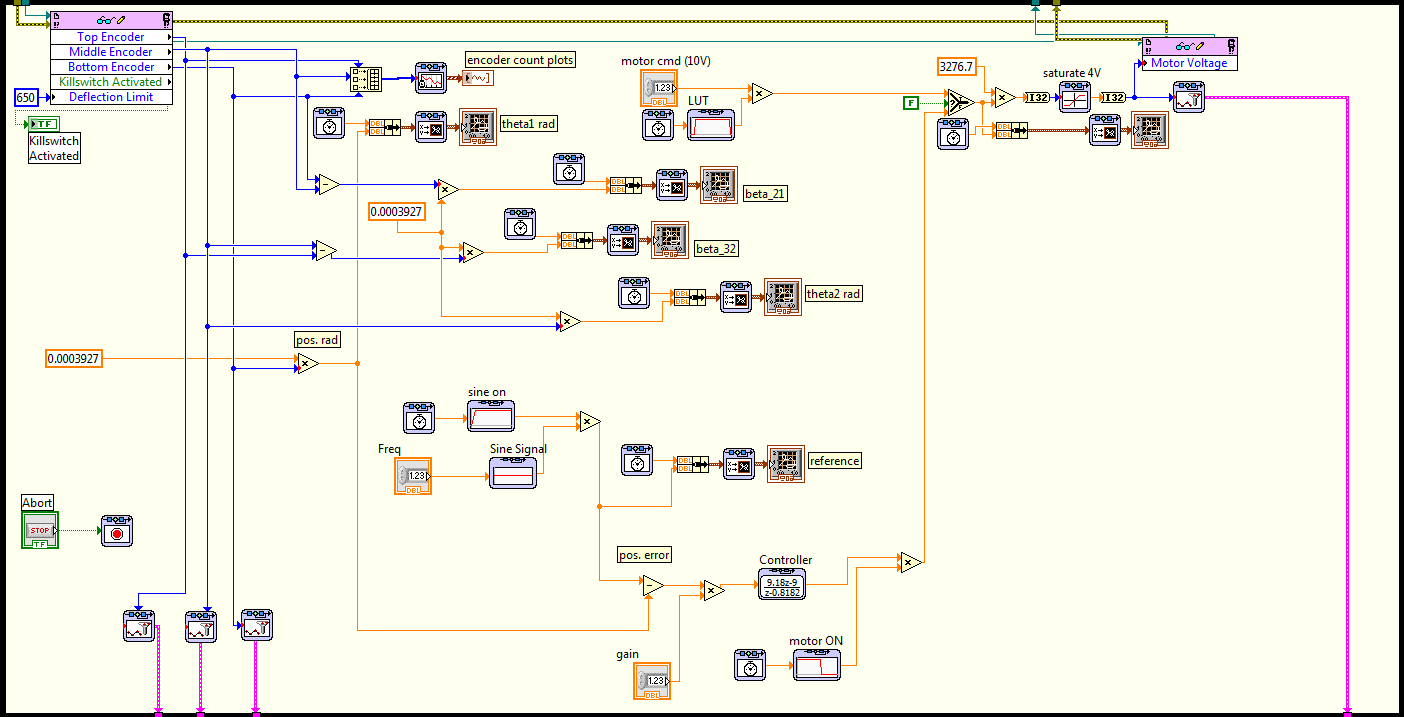
\includegraphics[scale=0.35]{labview}
                    \caption{Modified Labview Design}
                    \label{fig:labview}
            \end{figure}
    \subsection{Equations of Motion}
        The 3 disc TDS can be represented by the following system of equations:
        \begin{align}
            J_1\ddot{\Theta_1} &+ c_1\dot{\Theta_1} + k_1(\Theta_1 - \Theta_2) = bu \\
            J_2\ddot{\Theta_2} &+ c_2\dot{\Theta_2} + k_1(\Theta_2 - \Theta_1) + k_2(\Theta_2-\Theta_3) = 0 \\
            J_3\ddot{\Theta_3} &+ c_3\dot{\Theta_3} + k_2(\Theta_3 - \Theta_2) = 0
        \end{align}
    \subsection{Calculated System Values}
        The system values needed in order to design a functional controller a listed below:
        \begin{align}
            J_1 &=0.0115     &       J_2 &= 0.0064       &   J_3 &= 0.0064  \\
            b &= 0.305       &       k &= 2.55           &   C_1 &= 0.005   \\
            c_2 &= 0.0016    &       c_3 &= 0.0016       &       &          \\
        \end{align}
    \subsection{Controller}
        Using the state space representation of the E.O.M. we designed the following controller using SISO tool.
        \begin{equation}
            C_s = \frac{995.3 s^2 + 8423 s + 1036}{s^2 + 29.15 s + 103.6}
        \end{equation}
        This controller has a large DC gain of $~10$ and attempts to stabilize the system in a more aggressive manner. This method was chosen to reduce the magnitude of the instabilities at certain frequencies.
    \subsection{Matlab Plots}
        The majority of our controller design was conducted using SISO tool and viewing the root locus of the system. This allowed us to make the desired changes to the phase and gain margins and view the results in real time.
        \begin{figure}[H]
            \centering
            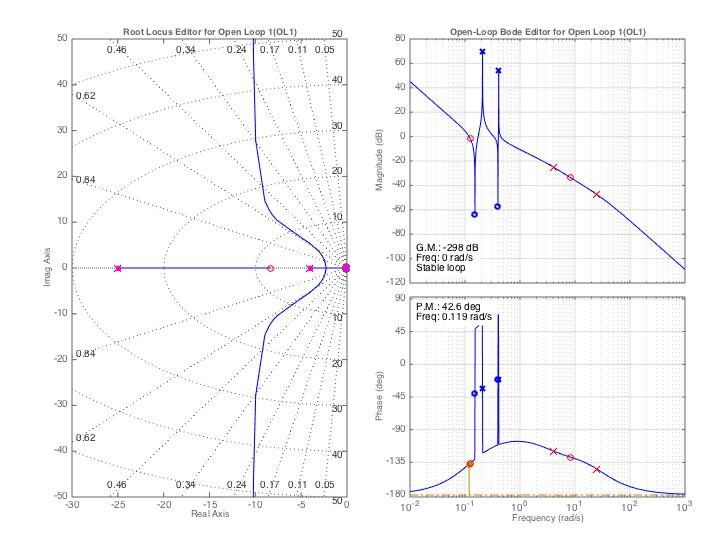
\includegraphics[scale=0.35]{r_locus}
            \caption{Root Locus}
            \label{fig:rlocus}
        \end{figure}
        We found it more beneficial to plot multiple bode plots on one graph. This allowed us to view the relation between different disc levels. As seen in the below plot, the middle disc should remain still at 3.2 Hz.
        \begin{figure}[H]
            \centering
            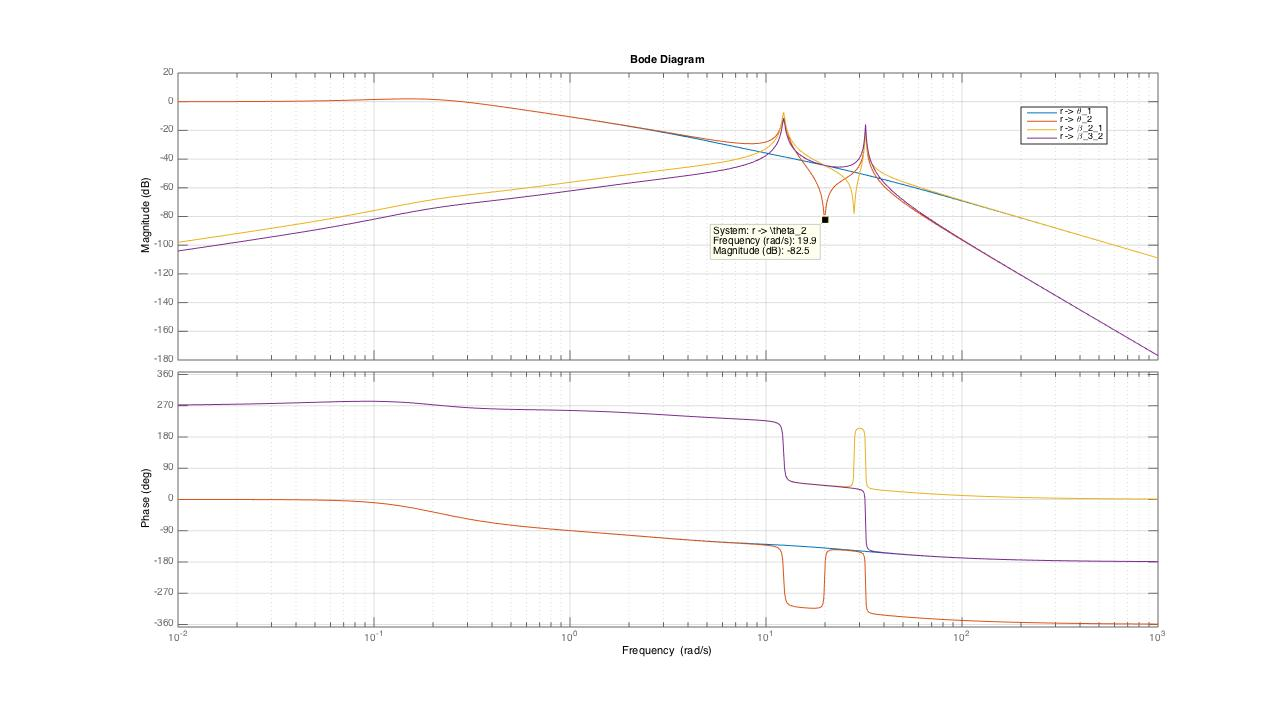
\includegraphics[scale=0.35]{bode_all}
            \caption{Combined Bode Plots}
            \label{fig:bode_all}
        \end{figure}
        In order to use the designed controller in Labview we first converted it to discrete time. The below plot shows the discrete time controller and the continuous time controller on the same plot. Clearly, the discrete time controller tracks the continuous reasonably well and should operate as desired.
        \begin{figure}[H]
            \centering
            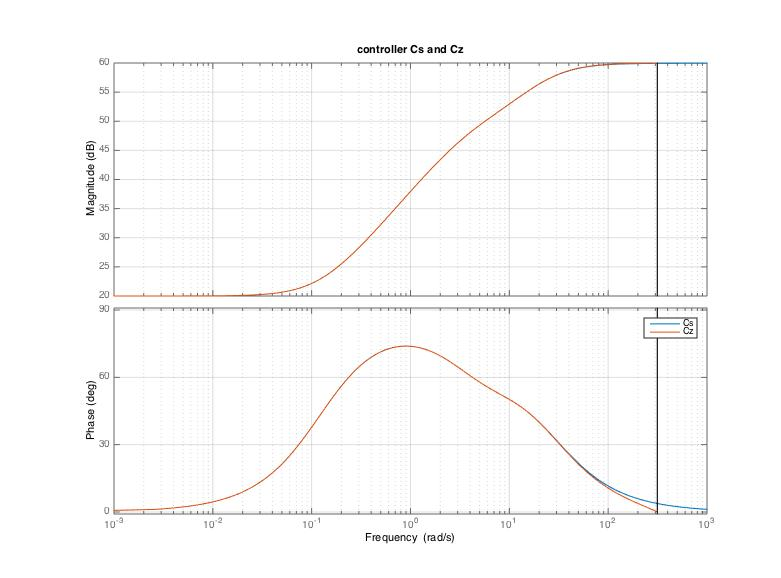
\includegraphics[scale=0.35]{Cs_Cz}
            \caption{Continuous vs. Discrete Controller}
            \label{fig:csCz}
        \end{figure}

\section{Controller Implementation on TDS}
    \subsection{Live System Results}
        After completing the above controller design we implemented the controller on the TDS. We at first encountered problems with the "kill switch" being activated each time we ran an experiment. The reason for this was the amplitude of the sinusoidal input and the speed at which the system attempted to reach the input frequency. To remedy the problem we reduced the amplitude of the sinusoid from 1 to 0.15 and changed the reference signal to start as a ramp rather than a step. This resolved the issue and we then conducted a frequency sweep of the system to determine if our Matlab analysis aligned with the actual results. As expected we were able to view the middle disc remaining in a stationary position at 3.2 Hz. Another important observation was the amount of gain we used in the controller design. With a DC gain of 10 the system responded abruptly to minor changes and at the resonant peaks the kill switch was quickly activated. Reducing the gain helped with this problem some but did not eliminate the issue.
    \subsection{Experimental Plots}
    The below plots show the response of the live system using our designed controller.

\section{Conclusion}
    This final lab was a good ending point for our exploration of the TDS system. We were able to design a controller that operates as desired with 3 discs attached to the TDS. Further exploration and time would allow us to design a more robus controller. Utilizing a SIMO or MIMO controller design would be much more accurate but unfortunately we did not have time to explore this option.

\end{document}
